\documentclass[a4]{scrartcl}

\usepackage[ngerman]{babel}
\usepackage[utf8]{inputenc}
\usepackage{mathtools}
\usepackage{amsmath}
\usepackage{amssymb}
\usepackage{geometry}
\usepackage{scrpage2}
\pagestyle{scrheadings}
\clearscrheadfoot


\geometry{
  paper=a4paper, % Change to letterpaper for US letter
  top=2cm, % Top margin
  bottom=1.5cm, % Bottom margin
  left=2cm, % Left margin
  right=3cm, % Right margin
  %showframe, % Uncomment to show how the type block is set on the page
}

\setlength{\parindent}{0em}

\ohead{\\
Pina Kolling}

\begin{document}


\section*{Vorlesung 1}

\begin{itemize}
    \item \textbf{Digitization}: Digitalisierung von Daten \\
    Die Umwandlung von analogen in digitale Produkte und Dienstleistungen
    \item \textbf{Digitalization}: Digitalisierung der Wertschöpfung \\
    Die Veränderung von Geschäftsprozessen durch digitale Technologien
    \item \textbf{Digitale Transformation}: \\
    Die Neuorganisation von Geschäftsmodellen und Industrien durch digitale Technologien
\end{itemize}

\ \\
\textbf{Digitalisierung}:
\begin{itemize}
    \item Abnehmende Distanz zwischen IT und Realität
    \item Moorsches Gesetz
    \item Kapselung von Funktionalitäten
    \item KI-Entwicklung 
\end{itemize}

\ \\
\textbf{Wirtschaftsinformatik}:

\begin{itemize}
    \item \textbf{Realwissenschaft}: \\
    Forschungsgegenstand sind reale Sachverhalte
    \item \textbf{Formalwissenschaft}: \\
    Abstrakte Inhalte als Forschungsgegenstand
    \item \textbf{Ingenieurwissenschaft}: \\
    Technik und Entwicklung dieser
\end{itemize}
 
 \ \\
\textbf{ Was ist Ziel der Wirtschaftsinformatik? }\\
 Die Gestaltung von sozial akzeptablen, technisch stabilen und ökonomisch nachhaltigen Informationssystemen.

\ \\

\begin{center}
    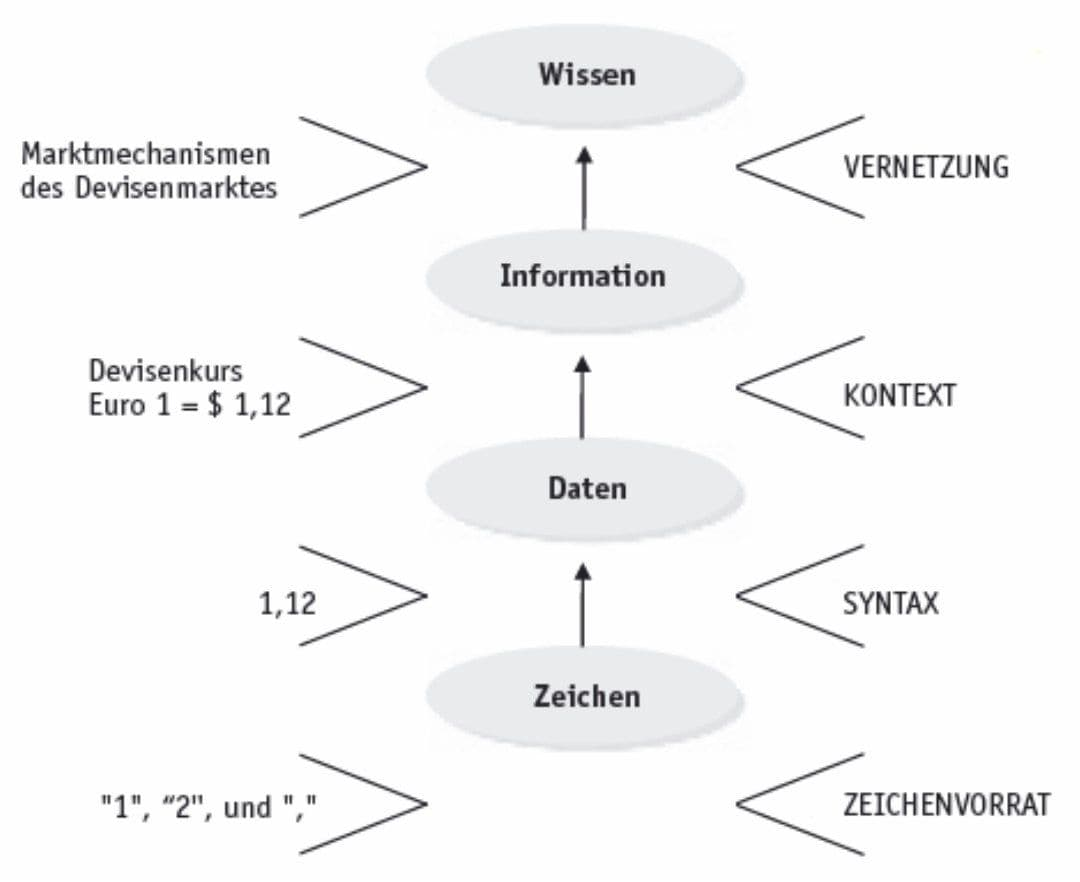
\includegraphics[width= 10cm]{digi.jpg}
\end{center}

\textbf{Informationslogistik}: \\ \\
Ziele: \\
\begin{itemize}
    \item richtige Information
    \item richtiger Zeitpunkt
    \item richtige Menge (so wenig wie möglich)
    \item richtiger Ort
    \item erforderliche Qualität (ausreichend)
\end{itemize}
\ \\
\textbf{Informationssystem}: \\
\\
Bei Informationssystemen handelt es sich um soziotechnische (Mensch-Maschine) Systeme, die menschliche und maschinelle Komponenten (Teilsysteme) umfassen, insbesondere einer Aufgabenerfüllungdienen und zum Ziel der optimalen Bereitstellung von Informationen, Koordination und Kommunikation nach wirtschaftlichen Kriterien eingesetzt werden.

\begin{itemize}
    \item erzeugt oder benutzt Informationen
    \item verbindet Akteure durch Kommunikationsbeziehungen miteinander
\end{itemize}

Grundfragen bei der Gestaltung von Informationssystemen:
\begin{itemize}
    \item Wozu wird die Information gebraucht?
    \item Wer soll wen über was informieren?
    \item Wann soll informiert werden?
    \item Wie soll informiert werden?
\end{itemize}

\ \\
\textbf{Ziele der Informationssysteme}:
\begin{itemize}
    \item Planung, Steuerung und Kontrolle in der Organisation unterstützen
    \item Geschäftsprozesse beschleunigen
    \item Qualität und Service verbessern
    \item Wettbewerbsvorteile generieren
\end{itemize}


\end{document}
